\documentclass[a4paper]{report}
\usepackage[utf8]{inputenc}
\usepackage[T1]{fontenc}
\usepackage{RJournal}
\usepackage{amsmath,amssymb,array}
\usepackage{booktabs}

%% load any required packages FOLLOWING this line

\usepackage{subfigure, enumitem}
\usepackage{url}
\usepackage{mdframed}


\newcommand{\bR}{ \mbox{\boldmath $R$} }
\newcommand{\bb}{ \mbox{\boldmath $b$} }
\newcommand{\bSigma}{ \mbox{\boldmath $\Sigma$} }
\newcommand{\bbeta}{ \mbox{\boldmath $\beta$} }
\newcommand{\bzero}{ \mbox{\boldmath $0$} }
\newcommand{\bone}{ \mbox{\boldmath $1$} }
%\newcommand{\CRANpkg}{\href{http://CRAN.R-project.org/package=#1}{\pkg{#1}}}

\begin{document}

%% do not edit, for illustration only
\sectionhead{Contributed research article}
\volume{14}
\volnumber{1}
\year{2022}
\month{March}
\setcounter{page}{269}

%% replace RJtemplate with your article
\begin{article}
  % !TeX root = RJwrapper.tex
\title{Power and Sample Size for Longitudinal Models in R -- The \pkg{longpower} Package and Shiny App}
\author{by Samuel Iddi and Michael C. Donohue}


\maketitle

\abstract{
Longitudinal studies are ubiquitous in medical and clinical research. Sample size computations are critical to ensure that these studies are sufficiently powered to provide reliable and valid inferences. There are several methodologies for calculating sample sizes for longitudinal studies that depend on many considerations including the study design features, outcome type and distribution, and proposed analytical methods. We briefly review the literature and describe sample size formulas for continuous longitudinal data.  We then apply the methods using example studies comparing treatment versus control groups in randomized trials assessing treatment effect on clinical outcomes. We also introduce a Shiny app that we developed to assist researchers with obtaining required sample sizes for longitudinal studies by allowing users to enter required pilot estimates. For Alzheimer's studies, the app can estimate required pilot parameters using data from the Alzheimer’s Disease Neuroimaging Initiative (ADNI). Illustrative examples are used to demonstrate how the package and app can be used to generate sample size and power curves. The package and app are designed to help researchers easily assess the operating characteristics of study designs for Alzheimer's clinical trials and other research studies with longitudinal continuous outcomes. Data used in preparation of this article were obtained from the Alzheimer's Disease Neuroimaging Initiative (ADNI) database (adni.loni.usc.edu).
}

\section{Introduction}

\label{sec1}

Longitudinal designs are generally preferred over cross-sectional research designs as they provide richer data and greater statistical power. As such, many biomedical and medical studies employ longitudinal designs to study changes over time in outcomes at the individual, group, or population level. Early in the design of a longitudinal experimental or natural history study, it is imperative to ensure that the study is adequately powered for its aims.  Inadequate sample sizes leads to invalid or inconclusive inference and squandered resources \citep{Lu_Methrotra_Liu(2009),Yan_Su(2006)}. On the other hand, oversampling squanders resources and exposes participants to unnecessary risks associated with the intervention \citep{Lu_Methrotra_Liu(2009)}. Thus, optimal sample size and power analysis have become important prerequisites for any quantitative research design. Not only are these required during the design phase of research, but it has also become mandatory for ethical, scientific, or economic justification in submissions to institutional review boards and research funding agencies.

Determining the right sample size for a study is not a straightforward task. Despite the plethora of sample size formulas for repeated measures \citep{Overall_Doyle(1994),Lui(1992),Rochon(1991), Guo_etal(2013)}, cluster repeated measures \citep{Liu_Shih_Gehan(2002)}, multivariate repeated measures \citep{Vonesh_Schork(1986),Guo_Johnson(1996)}, longitudinal research designs \citep{Lefante(1990)}, the tasks of gathering pilot estimates of the necessary parameters and getting the right software to carry out the computation can be challenging. Researchers commonly rely on formulas for very basic cross-sectional studies and adjust for attrition and other longitudinal design effects. Although such approaches can yield appropriate approximations, the ideal approach is to use a formula derived directly from the longitudinal model that researchers plan to eventually use on the study data.

\cite{Guo_etal(2013)} describe practical methods for the selection of appropriate sample size for repeated measures addressing issues of missing data, and the inclusion of more than one covariate to control for differences in response at baseline. Sample size formulas are refined depending on the specific situation and design features. For example, \cite{Hedeker_Gibbons_Waternaux(1999)} considered a sample size for longitudinal designs comparing two groups that accounted for participant attrition or drop-out. \cite{Basagana_Liao_Spiegelman(2011)} derived sample size formulas for continuous longitudinal data with time-varying exposure variables typical of observational studies. Ignoring time-varying exposure was demonstrated to lead to substantial overestimation of the minimum required sample size which can be economically disadvantageous. In non-traditional longitudinal designs such as designs for mediation analysis of the longitudinal study, further refinements to sample size formulas are needed to ensure that sufficient sample sizes are obtained \citep{Pan_etal(2018)}. However, these formulas usually require additional parameters such as exposure mean, variance, and intraclass correlations \citep{Basagana_Liao_Spiegelman(2011)}, mediation effect, number of repeated measures  \citep{Pan_etal(2018)}, covariance structures \citep{Rochon(1991)}, non-linear trends \citep{Yan_Su(2006)}, missing, attrition or dropout rates \citep{Roy_etal(2007), Lu_Luo_Chen(2008)}, among others.  Advanced sample size methods simultaneously handle several practical issues associated with the research design and complications that may arise during data collection. However, such methods are only available in commercial software \citep{NCSS(2021),nQuery(2021)}. 

Several R packages can be found on CRAN to compute sample size based on mixed-effect models and other specific designs depending on the area of applications. For example, \cite{Martin_etal(2011)} proposed a simulation-based power calculation and an R package \CRANpkg{pamm} for random regression models, a specific form of mixed-effect model that detects significant variation in individual or group slopes. In their approach, a power analysis was performed to detect a specified level of individual and environmental interactions within evolution and ecology applications. This is achieved by simulating power to detect a given covariance structure. Other simulation-based packages for power analysis are the \CRANpkg{SIMR} by \cite{Green_MacLeod(2016)} for linear and generalized linear mixed models and \CRANpkg{clusterPower} by \cite{Kleinman(2021)} for cluster-randomized and cross-over designs. \cite{Schoenfeld(2019)} developed a power and sample size package called \CRANpkg{LPower} \citep{Diggle_Liang_Zeger(1994)} to perform power analysis for longitudinal design accounting for attrition and different random effect specification. The approach requires the specification of a design matrix, and the variance-covariance matrix of the repeated measures \citep{Yi_Panzarella(2002)}. In pharmacokinetic study designs, \cite{Kloprogge_Tarning(2015)} developed the \CRANpkg{PharmPow} power calculation package for mixed study designs including crossover and parallel designs. Quite recently, other R packages for performing power analysis exist for different designs; for example the \CRANpkg{powerMediation} \citep{Qiu(2021)} for mediation effect, mean change for longitudinal study with 2-time points, the slope for simple Poisson regression, etc.; \CRANpkg{powerEQTL} \citep{Dong_etal(2021)} for unbalanced one-way ANOVA in a Bulk Tissue and Single-Cell eQTL Analysis; \CRANpkg{WebPower}  \citep{Zhang_Mai_Yang(2021)} for basic and advanced power correlation, proportion, $t$-test, one-way ANOVA, two-way ANOVA, linear regression, logistic regression, Poisson regression, mediation analysis, longitudinal data analysis, structural equation modeling, and multilevel modeling; among others. These packages were tailored towards very specific areas of application although the methods can be adapted and utilized for other disciplines. In terms of software applications, attempts have been made in recent times to implement power and sample size calculations in Shiny applications to facilitate easy usage. For example, \cite{Hemming_etal(2020)} developed an R Shiny app to conduct power analysis for several cluster designs including parallel, cross-over, and stepped-wedge designs. \cite{Schoemann_Boulton_Short(2017)} Shiny application conducts power analysis for mediation model, and \cite{Hu_Qu(2021)} performs sample size and power calculations for a random coefficient regression model (RCRM) and a two-stage mixed-effects model.

As the analysis model and associated sample size formula become more sophisticated, estimating the parameters required by the formula becomes more challenging. A major hurdle to overcome is the availability of pilot data to inform these parameters. To assist Alzheimer's researchers with this challenge, we have developed a power and sample size Shiny app for Alzheimer's clinical trials. The app implements formulas for the linear mixed-effects model and mixed model for repeated measures \citep[MMRM; ][]{Lu_Luo_Chen(2008)} allowing the user to input their pilot estimates, or allow the app to generate pilot estimates using data from the Alzheimer's Disease Neuroimaging Initiative \citep[ADNI; ][]{Weiner_etal(2015)}.

\section{Review of methods}
\label{sec2}
Continuous outcomes in clinical trial data collected longitudinally over time are commonly analyzed using linear mixed models \citep[LMM; ][]{Laird_Ware(1982)} or MMRM \citep{Mallinckrodt_etal(2001),Mallinckrodt_etal(2003)}. Before such trials, it is necessary to estimate the required sample size for a given treatment effect with desired power and Type I error. Various sample size approaches for longitudinal data have been proposed. We review a few of the most commonly used methods applied in Alzheimer’s disease trials with continuous outcomes.


\subsection{Sample size computation based on the linear mixed-effects model}
\label{model}
Several sample size approaches have been developed by different authors. \cite{Diggle_etal(2002)} proposed sample size formulas for two approaches to continuous longitudinal outcomes, one that assumes a constant mean over time and compares the average response over time between groups, and another that assumes a linear change over time and compares the mean rate of change or slope difference between groups. In either case, the null hypothesis is that there is no difference between groups. Suppose that $Y_{ij}$ is the response for participant $i$ taken at time $j$. To compare the average response between two groups (e.g. group $A$ receiving active treatment and group $B$ receiving control) across time, consider the model
$$Y_{ij}=\beta_0+\beta_1T_i+\epsilon_{ij}$$
where $T_i$ is the treatment indicator which is coded 1 for participants in group $A$ and 0 for participants in group $B$, and $\epsilon_{ij}$ the error term for subject, $i$ at time $j$, which is normally distributed with common variance, $\sigma^2$. The sample size required per group to detect an average response between the two groups, $\delta$, is given by
$$m=\frac{2(Z_{1-\alpha/2}+Z_{P})^2\sigma^2(1+(J-1)\rho)}{J\delta^2}$$
where $\alpha$ is the type I error rate, $P$ is the level of power, and $\mbox{corr}(Y_{ij},Y_{ik})=\rho$ for all $j\neq k$.

To test difference in the slopes or average rate of change between the two groups, consider the parameterization:
$$Y_{ij}=\beta_{0A}+\beta_{1A}t_{ij}+\epsilon_{ij}, i=1,2,\dots,m; j=1,2,\dots,J.$$
A similar parameterization can be specified for group $B$ with parameters $\beta_{0B}$, and $\beta_{1B}$ representing the intercept and slope. The parameters $\beta_{1A}$ and $\beta_{1B}$ are the rate of change of the outcome for groups $A$ and $B$, respectively. Assume that $\mbox{var}(\epsilon_{ij})=\sigma^2$ and $\mbox{corr}(Y_{ij},Y_{ik})=\rho$ for all $j\neq k$. If the outcome of each participant is measured at the same time, $t_j$, then the sample size per group needed to detect a difference in the rate of change for each group, $\Delta=\beta_A-\beta_B$, is given by
$$m=\frac{2(Z_{1-\alpha/2}+Z_{P})^2\sigma^2(1-\rho)}{Js^2_t\Delta^2}$$
where $\alpha$ is the type I error rate, $P$ is the power, and $s^2_t=\frac{\sum (t_j-\bar{t})}{J}$ is the within-participant variance of $t_j$. 

Another sample size computation approach for correlated data is derived by \cite{Liu_Liang(1997)} to detect differences in the average response between two groups. This approach derived sample size following the generalized estimating equation \citep{Liang_Zeger(1986)} approach. Thus, different outcomes types can be handled. A special case is for a continuous response measured repeatedly over time and modeled using a linear model. Consider the model $$Y_{ij}=\beta_0+\beta_1T_i+\epsilon_{ij}, i=1,2,\dots, N,j=1,2,\dots,J$$
where $T_i$ is the treatment indicator, $\epsilon_{ij}$ is the error term assumed to follow a multivariate normal distribution with a mean vector of zeros, $\bzero$, and covariance matrix, $\sigma^2\bR$ and $\bR$ is a $J\times J$ working correlation matrix. Different covariance structures such as independent, exchangeable, auto-regressive, and unstructured can be assumed. To estimate the total sample size required, $N$ for a given significance level ($\alpha$) and pre-specified nominal power, $P$, the following formula is used:
$$N=\frac{\left(Z_{1-\alpha/2}+Z_{P}\right)^2\sigma^2}{\pi_A\pi_B(\beta_1^2\bone\bR^{-1}\bone)}$$
where $\pi_A$ and $\pi_B$ represent the proportion of observations in the control and treated groups, respectively. By assuming an exchangeable working correlation matrix, this formula reduces to
$$N=\frac{\left(Z_{1-\alpha/2}+Z_{P}\right)^2\sigma^2[1+(J-1)\rho]}{\pi_A\pi_B\beta_1^2J}.$$  
It can be observed that for equal proportion of participants in each group i.e. $\pi_A=\pi_B=\frac{1}{2}$,  the formula for the sample size per group is equivalent to the sample size formula for difference in average response between groups by \cite{Diggle_etal(2002)} above. An appealing aspect of \cite{Liu_Liang(1997)} approach is that it can allow for unequal allocation to the two groups, and different outcome types are considered. 

Another approach is based on the LMM analysis \citep{Fitzmaurice_Laird_Ware(2004)} comparing mean rate of change between groups \citep{Ard_Edland(2011), Zhao_Edland(2020)}. Consider the LMM $$Y_{ij}=X'_{ij}\bbeta+b_{0i}+b_{1i}t_{ij}+\epsilon_{ij}$$
where $X_{ij}$ denotes a vector of indicator variables (treatment, time, and interaction terms), $\bb_i=(b_{0i},b_{1i})'\sim N\left(\left(\begin{array}{cc}
0\\0
\end{array}\right),\left[\begin{array}{cc}
\sigma^2_{b_0}&\sigma_{b_{0},b_{1}}\\
\sigma_{b_{0},b_1}&\sigma^2_{b_1}
\end{array}\right]\right)$ are random participant-specific effects, and $\epsilon_{ij}\sim N(0,\sigma^2_e)$ are the residual errors. The random terms, $\bb_i$ and $\epsilon_{ij}$ are assumed to be independent of each other. Following this model specification, \cite{Ard_Edland(2011)} proposed a total sample size formula given by
$$N=\frac{4\left(Z_{1-\alpha/2}+Z_{P}\right)^2}{\Delta^2}\left[\sigma^2_{b_1}+\frac{\sigma^2_e}{\sum (t_j-\bar{t})^2}\right]$$
where $t_j$ indexes the times at which measures are made assuming all participants are
observed at the same time points, $\bar{t}$ is the mean of the times, $\sigma^2_{b_1}$ is the variance of the participant-specific random slope, and $\Delta$ is the difference in mean rate of change in treatment versus control group to be detected. For a random-intercept mixed-effect model, the total sample size formula reduces to 
$$N=\frac{4\left(Z_{1-\alpha/2}+Z_{P}\right)^2}{\Delta^2}\left[\frac{\sigma^2_e}{\sum (t_j-\bar{t})^2}\right].$$
This sample size formula does not account for the correlation between the random intercept and slope, a limitation that can be mitigated by a recent approach by \cite{Hu_Mackey_Thomas(2021)}.

\subsection{Sample size computation based on the mixed model for repeated measures (MMRM)}
\label{model2}
An alternative approach is to treat time as a categorical variable. This approach, common in trials of treatments of Alzheimer’s and other therapeutic areas, is often referred to as the MMRM \citep{Mallinckrodt_etal(2001),Mallinckrodt_etal(2003),Lane(2008)}. The approach to fitting the MMRM is similar to that for other linear mixed-effect models for longitudinal or repeated measures except the unstructured modelling of time – treated as a categorical variable, and the specification of a within-participant correlation structure to account for association among the repeated measurements. The MMRM provides an estimate of the mean response for each time point category, for each group, and the resulting mean trajectory over time is unconstrained. The primary test statistic is usually the estimated group difference at the final time point. The null hypothesis is again that there is no difference between groups.

Suppose that $Y_{ij}$ is the $j$th measurement taken of participant $i; i=1,2,\dots,N$ at time, $t_{ij}$ and $T_i$ represents treatment or group indicator. Assuming we have two groups, $a; =(A,B)$, let $n_{a_j}$ be the number of participants at time $j=1,2,\dots,J$ for group $a$. Thus, at time point 1, the total number of participants is $n_{A1}+n_{B1}$.
The response variable is assumed to follow a multivariate normal distribution with mean, variance-covariance and correlation matrix given respectively as 
\begin{eqnarray*}
E(Y_{ij}|T_i=a)&=&\mu_{aj}\\
cov(Y_{ij}, Y_{ik}|T_i=a)&=&\sigma_{ajk}=\bSigma_a\\
corr(Y_{ij}, Y_{ik}|T_i=a)&=&\frac{\sigma_{jk}}{\sigma_j\sigma_k}=\bR
\end{eqnarray*}
where $\sigma_j=\sigma_{jj}^{\frac{1}{2}}$. It is common to assume that the variance-covariance matrix is the same for each group in which case we can have $\bSigma_A=\bSigma_B=\bSigma$. Different correlation structures, $\bR$, can be assumed (eg., compound symmetry, autoregressive and unstructured). The sample size formula for MMRM \citep{Lu_Luo_Chen(2008)} can account for the attrition rate at each time point. Define the attrition rate $\zeta_{aj}=1-r_{aj}$, where $r_{aj}=\frac{n_{aj}}{n_{a1}}$ is the retention rate at time point, $j$. The sample size for group $A$ needed to achieve a power, $P$, at a significance level, $\alpha$ is given by $$n_{A1}=(\psi_A+\lambda\psi_B)(Z_{1-\alpha/2}+Z_{P})^2\frac{\sigma^2_J}{\delta_J}$$
where $\lambda=\frac{n_{A1}}{n_{B1}}$ is called the allocation ratio, $\delta_J$ is the effect size (difference in mean response between the two groups) at the last time point, $J$, and $\psi_a$ is  the $(J, J)$th component of the variance inflation factor, $I_a^{*-1}$ defined with respect to an estimation of the $\mu_{aj}$ for treatment group, $a$. Specifically, $\psi_a=\left[I_a^{*-1}\right]_{JJ}$ where $$I_a^*=\sum_{j=1}^{J}(r_{a,j}-r_{a,j+1})\begin{bmatrix}
\bR_j^{-1}&0_{j\times (J-j)}\\0_{(J-j)\times j}&0_{(J-j)\times (J-j)}
\end{bmatrix}$$
The total sample size at the first time point is therefore given by $$n_{A1}+n_{B1}=(1+\lambda^{-1})(\psi_A+\lambda\psi_B)(Z_{1-\alpha/2}+Z_{P})^2\frac{\sigma^2_J}{\delta_J}.$$


\subsection{The \CRANpkg{longpower} package}
\label{model3}
The aforementioned sample size approaches have been implemented in an R package, \CRANpkg{longpower} \citep{Donohue_Edland(2020)}, that can be found on CRAN via the URL \url{https://cran.r-project.org/web/packages/longpower/index.html}. The package also contains functions which translate pilot mixed effect model parameters (e.g. random intercept and/or slope) into marginal model parameters so that the formulas of \cite{Diggle_etal(2002)}  or \cite{Liu_Liang(1997)} or \cite{Lu_Luo_Chen(2008)} formula can be applied to produce sample size calculations for two sample longitudinal designs assuming known variance.

\subsection{A web-based app}
\label{model4}
The interactive Shiny \citep{RShiny(2021)} application available from the URL \url{https://atrihub.shinyapps.io/power/} is an interface to the \pkg{longpower} package developed to easily generate sample size and conduct power analysis for a longitudinal study design with two-group comparisons for a continuous outcome. The app similarly implements the sample size formula of \cite{Liu_Liang(1997)} and \cite{Diggle_Liang_Zeger(1994),Diggle_etal(2002)} using functions in the \pkg{longpower} package. A novel feature of the app is that  it can generate required pilot estimates by sourcing data from the Alzheimer's Disease Neuroimaging Initiative (ADNI).

\section{Illustrations}
\label{sec3}
\subsection{Illustration of the \pkg{longpower} package}
ADNI is a population-based longitudinal cohort study that follows study participants to collect data on their clinical, cognitive, imaging including MRI and PET images, genetic, and biochemical biomarkers. The study was designed to discover, optimize, standardize, and validate clinical trial measures and biomarkers that are used in AD clinical research. This multi-site longitudinal study runs at about 63 sites in the US and Canada and began in 2004. All the data generated from the ADNI study are entered into a data repository hosted at the Laboratory of Neuroimaging (LONI) at the University of Southern California, the LONI Image \& Data Archive (IDA). The data can be freely accessed upon request. Apart from the many uses of the data for advancing knowledge for AD trials \citep{Weiner_etal(2015)}, this big data resource can be used to improve study design. Specifically, in this paper, the data is used to generate pilot estimates for the computation of sample size and power.

We consider an Alzheimer's disease example using ADAS-Cog \citep{rosen1984alzheimer} pilot estimates from the ADNI database. Suppose that we want to compute the sample size required to detect an effect of 1.5 at the 5\% level of significance and 80\% power. The LMM fit to ADNI data has an estimated variance of random slope for group A (placebo or control group) of 74, and a residual variance of 10. Assuming study visits at (0.00, 0.25, 0.50, 0.75, 1.00, 1.25, 1.50) years, the sample size using the `edland' approach can be obtained by using the \code{edland.linear.power()} functions in the \pkg{longpower} R package as follows. 


	\begin{example}
> t = seq(0,1.5,0.25)
> edland.linear.power(delta=1.5, t=t, sig2.s = 24, sig2.e = 10, sig.level=0.05, 
power = 0.80)

Zhao and Edland, in process 

N = 414.6202
n = 207.3101, 207.3101
delta = 1.5
t = 0.00, 0.25, 0.50, 0.75, 1.00, 1.25, 1.50
p = 0, 0, 0, 0, 0, 0, 1
p_2 = 0, 0, 0, 0, 0, 0, 1
sig2.int = 0
sig.b0b1 = 0
sig2.s = 24
sig2.e = 10
sig2.int_2 = 0
sig.b0b1_2 = 0
sig2.s_2 = 24
sig2.e_2 = 10
sig.level = 0.05
power = 0.8
alternative = two.sided

NOTE: N is *total* sample size and n is sample size in *each* group 

	\end{example}

An alternative approach is to use \code{lmmpower()} and specify the argument \code{method="edland"} in the following way.


\begin{example}
> lmmpower(delta=1.5, t=t, sig2.s = 24, sig2.e = 10, sig.level=0.05, 
power = 0.80,method="edland")

Zhao and Edland, in process 

N = 414.6202
n = 207.3101, 207.3101
delta = 1.5
t = 0.00, 0.25, 0.50, 0.75, 1.00, 1.25, 1.50
p = 0, 0, 0, 0, 0, 0, 1
p_2 = 0, 0, 0, 0, 0, 0, 1
sig2.int = 0
sig.b0b1 = 0
sig2.s = 24
sig2.e = 10
sig2.int_2 = 0
sig.b0b1_2 = 0
sig2.s_2 = 24
sig2.e_2 = 10
sig.level = 0.05
power = 0.8
alternative = two.sided

NOTE: N is *total* sample size and n is sample size in *each* group 
\end{example}

The Diggle and Liu \& Liang approaches can be applied with the \code{diggle.linear.power()} and \\
\code{lui.liang.linear.power()} functions, respectively. The \code{lmmpower()} functions can be used for either approach with the appropriate specification of the \code{`method'} argument. 

The second illustrative example is the hypothetical clinical trial discussed in \cite{Diggle_etal(2002)}. Suppose that we are interested in testing the effect of a new treatment in reducing blood pressure through a clinical trial. The investigator is interested in randomizing participants between a control and active treatment group to have equal size. Three visits are envisaged with assessments planned at years 0, 2, and 5. Thus, $n=3$ and $s^2_x=4.22$. Assuming a type I error rate of 5\%, power of 80\% and smallest meaningful difference of 0.5 mmHg/year, we want to determine the number of participants needed for both treated and control groups for varying correlations (0.2, 0.5 and 0.8) and response variance (100, 200, 300).



\begin{example}
> n <- 3
> t <-  c(0,2,5)
> rho <-  c(0.2, 0.5, 0.8)
> sigma2 <-  c(100, 200, 300)
> tab = outer(rho, sigma2,
+             Vectorize(function(rho, sigma2){
+               ceiling(diggle.linear.power(
+                 delta=0.5,
+                 t=t,
+                 sigma2=sigma2,
+                 R=rho,
+                 alternative="one.sided",
+                 power = 0.80)$n[1])}))
> colnames(tab) = paste("sigma2 =", sigma2)
> rownames(tab) = paste("rho =", rho)
> tab
sigma2 = 100 sigma2 = 200 sigma2 = 300
rho = 0.2          313          625          938
rho = 0.5          196          391          586
rho = 0.8           79          157          235
\end{example}

The above code reproduces the table on page 29 of \cite{Diggle_etal(2002)}. We also reproduce the table on page 30 of \cite{Diggle_etal(2002)} for detecting a difference in average response between two groups through the method by \cite{Liu_Liang(1997)} as follows:

\begin{example}
> u = list(u1 = rep(1,n), u2 = rep(0,n)) #a list of covariate vectors or 
   matrices associated with the parameter of interest
> v = list(v1 = rep(1,n), v2 = rep(1,n)) #a respective list of covariate 
vectors or matrices associated with the nuisance parameter
> rho = c(0.2, 0.5, 0.8) #correlations
> delta = c(20, 30, 40, 50)/100 #effect size
> tab = outer(rho, delta,Vectorize(function(rho, delta){
+   ceiling(liu.liang.linear.power(
+     delta=delta, u=u, v=v,
+     sigma2=1,
+     R=rho, alternative="one.sided",
+     power=0.80)$n[1])}))
> colnames(tab) = paste("delta =", delta)
> rownames(tab) = paste("rho =", rho)
> tab
delta = 0.2 delta = 0.3 delta = 0.4 delta = 0.5
rho = 0.2         145          65          37          24
rho = 0.5         207          92          52          33
rho = 0.8         268         120          67          43
\end{example}

The sample size formula for the MMRM approach is also implemented in the \pkg{longpower} package's \code{power.mmrm()} function. To illustrate how this approach is implemented, consider a hypothetical example with a correlation matrix having 0.25 as off-diagonal entries (exchangeable), a retention vector (1, 0.90,0.80,0.70) and standard deviation of 1, for group A. Assuming these values to be the same for group B, then the sample size required to detect an effect size of 0.5 at 5\% level of significance and 80\% power is computed as follows:


\begin{example}
> Ra <- matrix(0.25, nrow = 4, ncol = 4)
> diag(Ra) <- 1 #exchangeable correlation matrix for group A
> ra <- c(1, 0.90, 0.80, 0.70)#retention in group A
> sigmaa <- 1 #standard deviation for group A
> power.mmrm(Ra = Ra, ra = ra, sigmaa = sigmaa, delta = 0.5, power = 0.80)

Power for Mixed Model of Repeated Measures (Lu, Luo, & Chen, 2008) 

n1 = 86.99175
n2 = 86.99175
retention1 = 1.0, 0.9, 0.8, 0.7
retention2 = 1.0, 0.9, 0.8, 0.7
delta = 0.5
sig.level = 0.05
power = 0.8
alternative = two.sided
\end{example}
Suppose the allocation ratio is 2, then the function argument \code{lambda=2} can be added. 

\subsection{Illustration of the Shiny app}
We demonstrate how the app is used to perform power analysis by inputting user-specified values and a specific sample size approach. We make use of the values shown in Table~\ref{parameters}. For the MMRM method, we specify the options assuming an exchangeable correlation structure.  

\begin{table}[ht]
	\caption{Parameter values considered in Shiny app demonstrations. Each row represents a different parameter and the values considered for the linear mixed model (LMM, left column) and the mixed model for repeated measures (MMRM, right column) demonstrations. The "-" indicates the parameter is "not applicable" for the given model.}\label{parameters}
	\begin{tabular}{lcc}
		\hline\hline
		Parameter&	LMM&	MMRM\\
		\hline
		Start time&	0&1\\	
		End time&	1.5	&4\\
		Timestep&	0.5	&1\\
		Type I error rate&	0.05&0.05	\\
		Effect size	&1.5&-	\\
		Estimate of variance of random intercept&	55	&-\\
		Estimate of variance of random slope&	22&	-\\
		Estimate of covariance of random intercept and slope&	29	&- \\
		Estimate of the error variance&	10	&-\\
		Standard deviation of observation in group A&	-&	1\\
		Standard deviation of observation in group B&	-&	1\\
		Exchangeable correlation&-&		0.25\\
		Allocation ratio&	1&2	\\
		\hline\hline
	\end{tabular}
\end{table}
	
For the ADNI-based pilot estimate generator, we select the full range of values for some selected variables (See Figure~\ref{ADNIbase}). 

\subsubsection{App menus and contents}
The app has three main menus on the sidebar. The first menu has two sub-menus which let the user perform power and sample size calculations based on longitudinal designs when necessary pilot estimates are known. The first submenu, the default, accepts user-specified inputs and generates a graphical output and summary of the inputs. In the `input' box, as shown in Figure~\ref{LMMinput}a, users are aided with the selection of their inputs through widgets such as select input, numerical input, slider input, and radio button to facilitate the user selection. The select input for `Analysis Type' allows the user to select whether the user desires to determine power or sample size. Input parameters that are not applicable for a given selection or are not applicable for the selected sample size method are grayed out to enhance the user experience. For example, the allocation ratio input widget is grayed out when the `diggle' and `liuliang' procedures are selected. The `output' box, shown in Figure~\ref{LMMinput}b, displays a graph of power versus sample size, a note on the method for the sample size computation, and a summary of the selected inputs by the user. The second submenu enables the user to conduct power analysis based on the MMRM methodology. Widgets such as select inputs, slider inputs, numerical inputs, and radio buttons display the current values of the model parameter in the `input' box (See Figure~\ref{MMRMinput}a). As the MMRM requires the specification of an association structure and a vector of the retention rates, the app display vectors, and matrix inputs widgets. The size of these widgets depends on users' choice of the number of time points for the study. However, these widgets are not reactive, and therefore the user must use the ``Update/Enter" action button when changes are made to the number of time points to update the vector and matrix input widgets. The corresponding graphical and summary outputs are reactively displayed within the `output' box, immediately below the `input’ box (See Figure~\ref{MMRMinput}b). 

\begin{figure}[ht]
	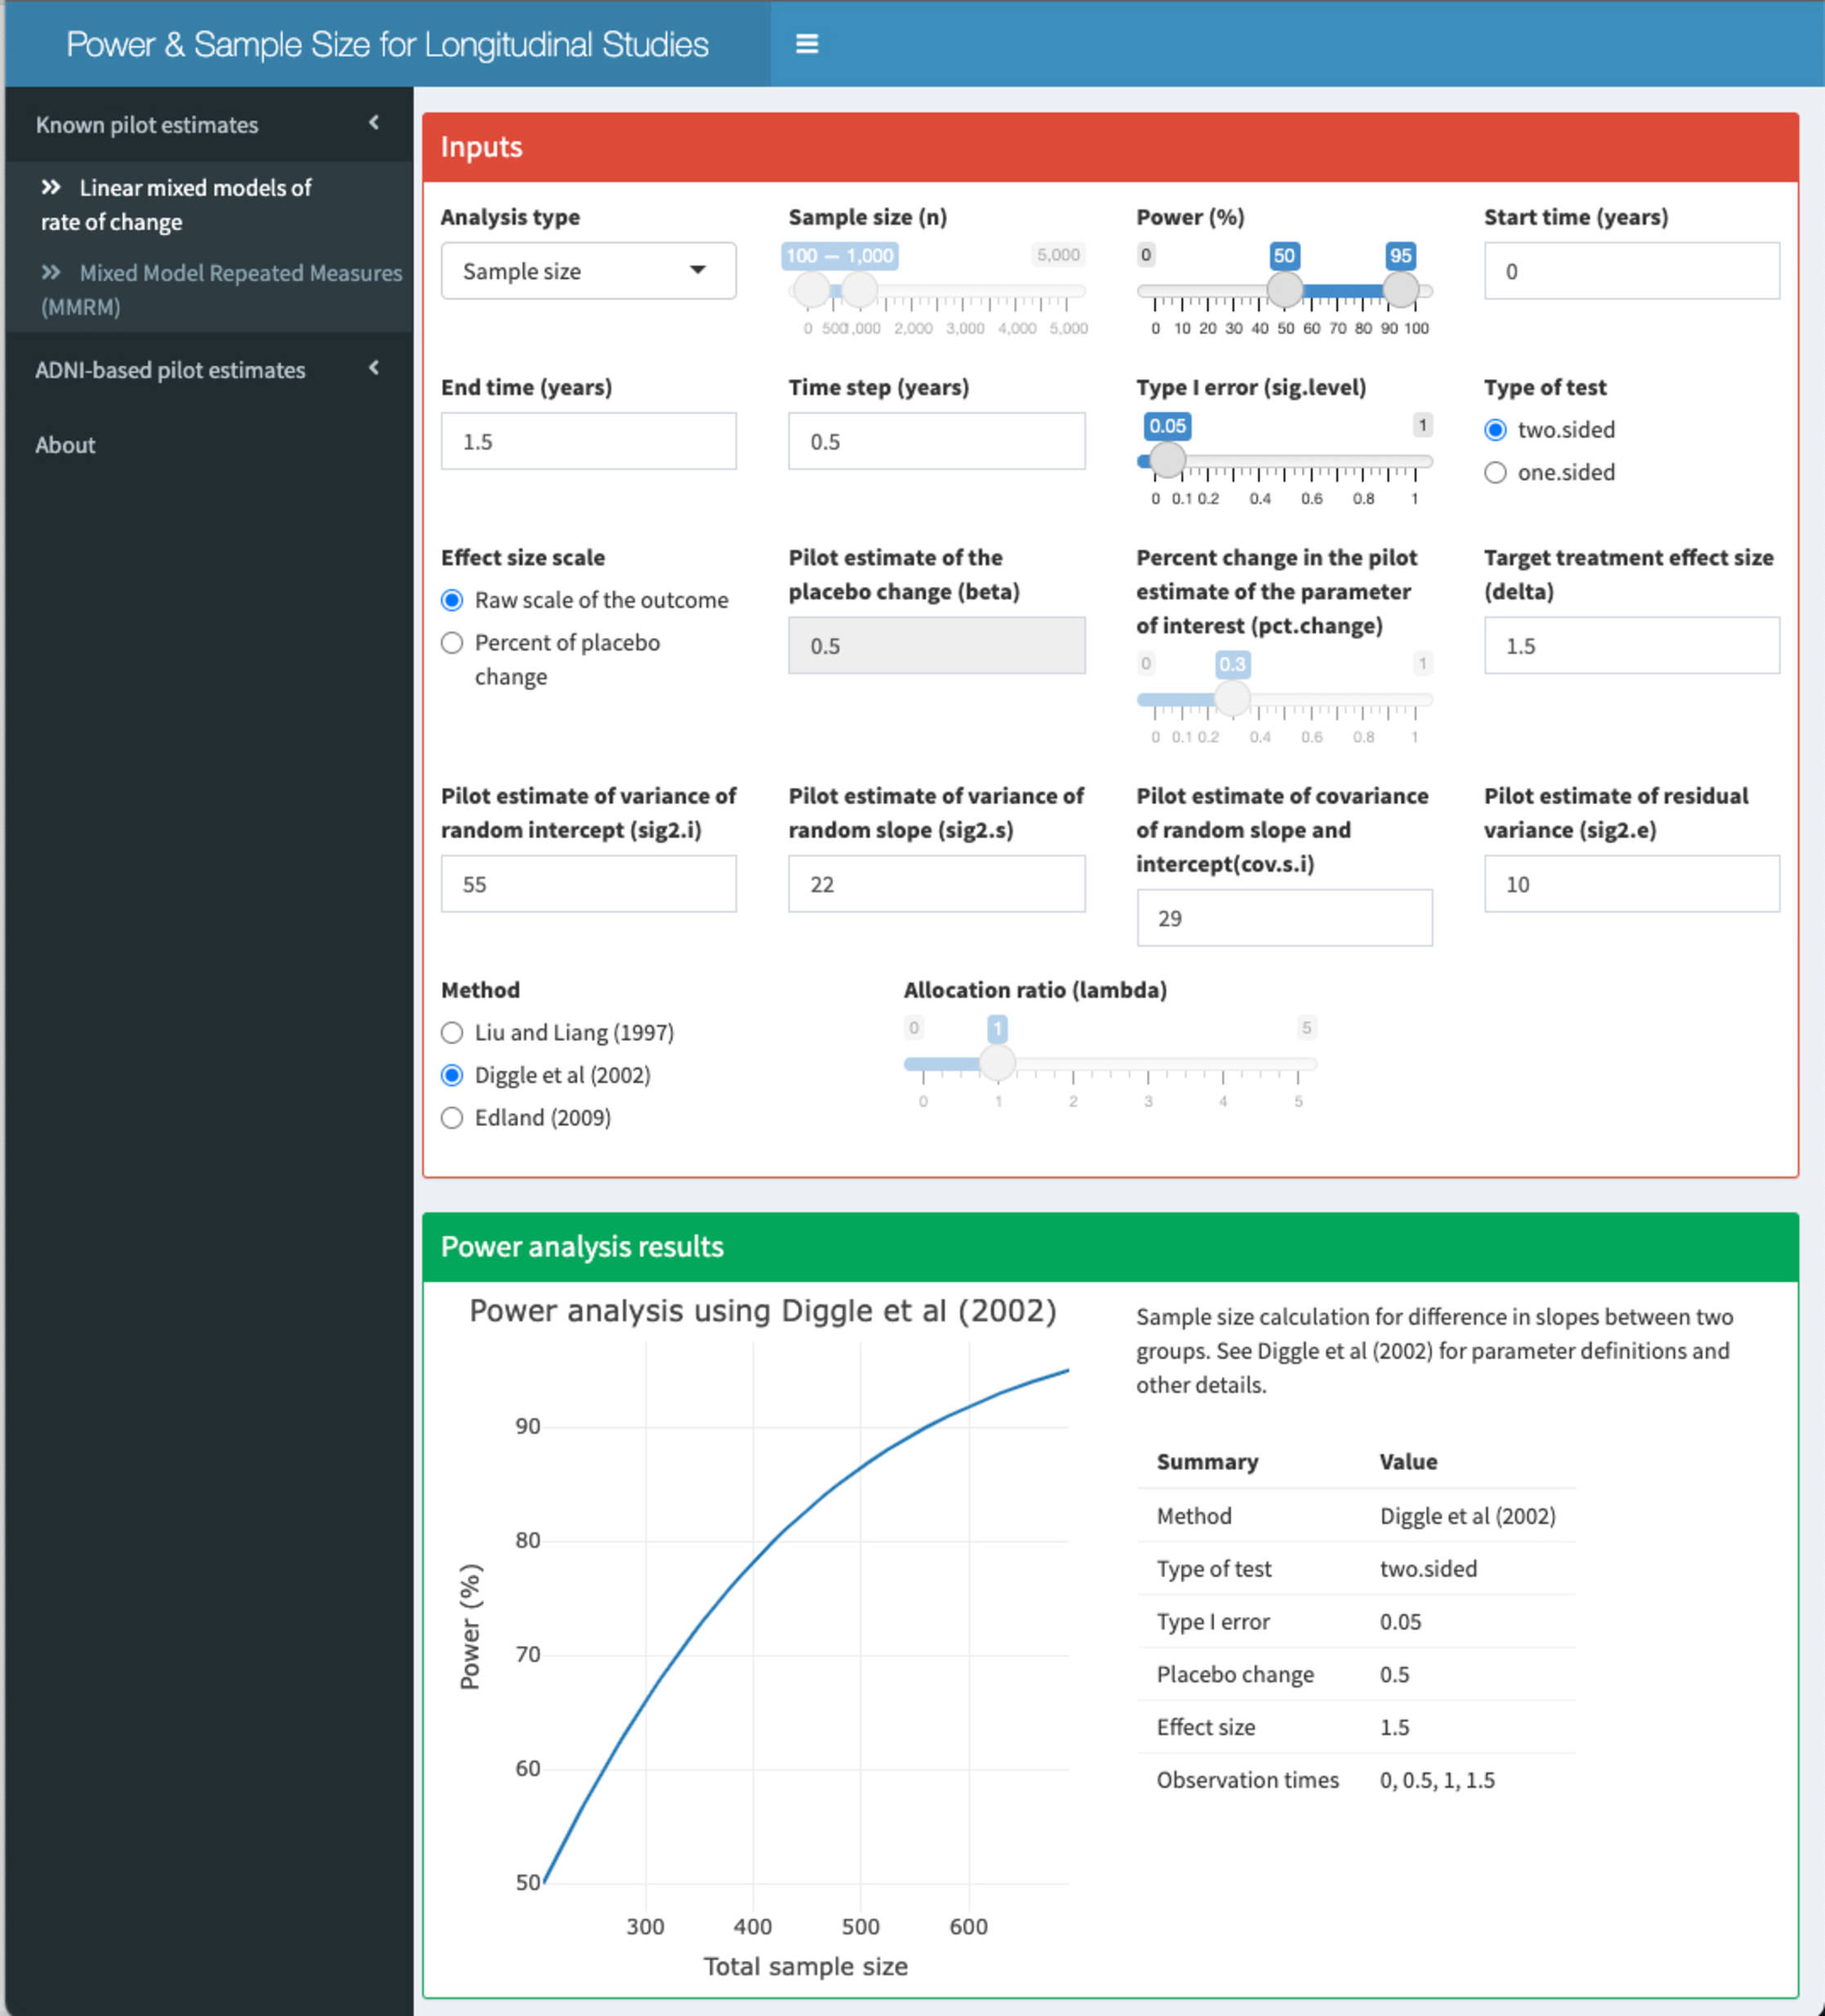
\includegraphics[width=14cm]{Figures/LMM-screenshot.pdf}\\
	\caption{Screenshot of Shiny app menu for linear mixed models (LMM) of rates of change. The red box (top) denotes an area where user input of pilot estimates and study design features is required. Output, including a power curve and a summary table of study design characteristics, is displayed in the green box (bottom).}\label{LMMinput}
\end{figure}

\begin{figure}[ht]
	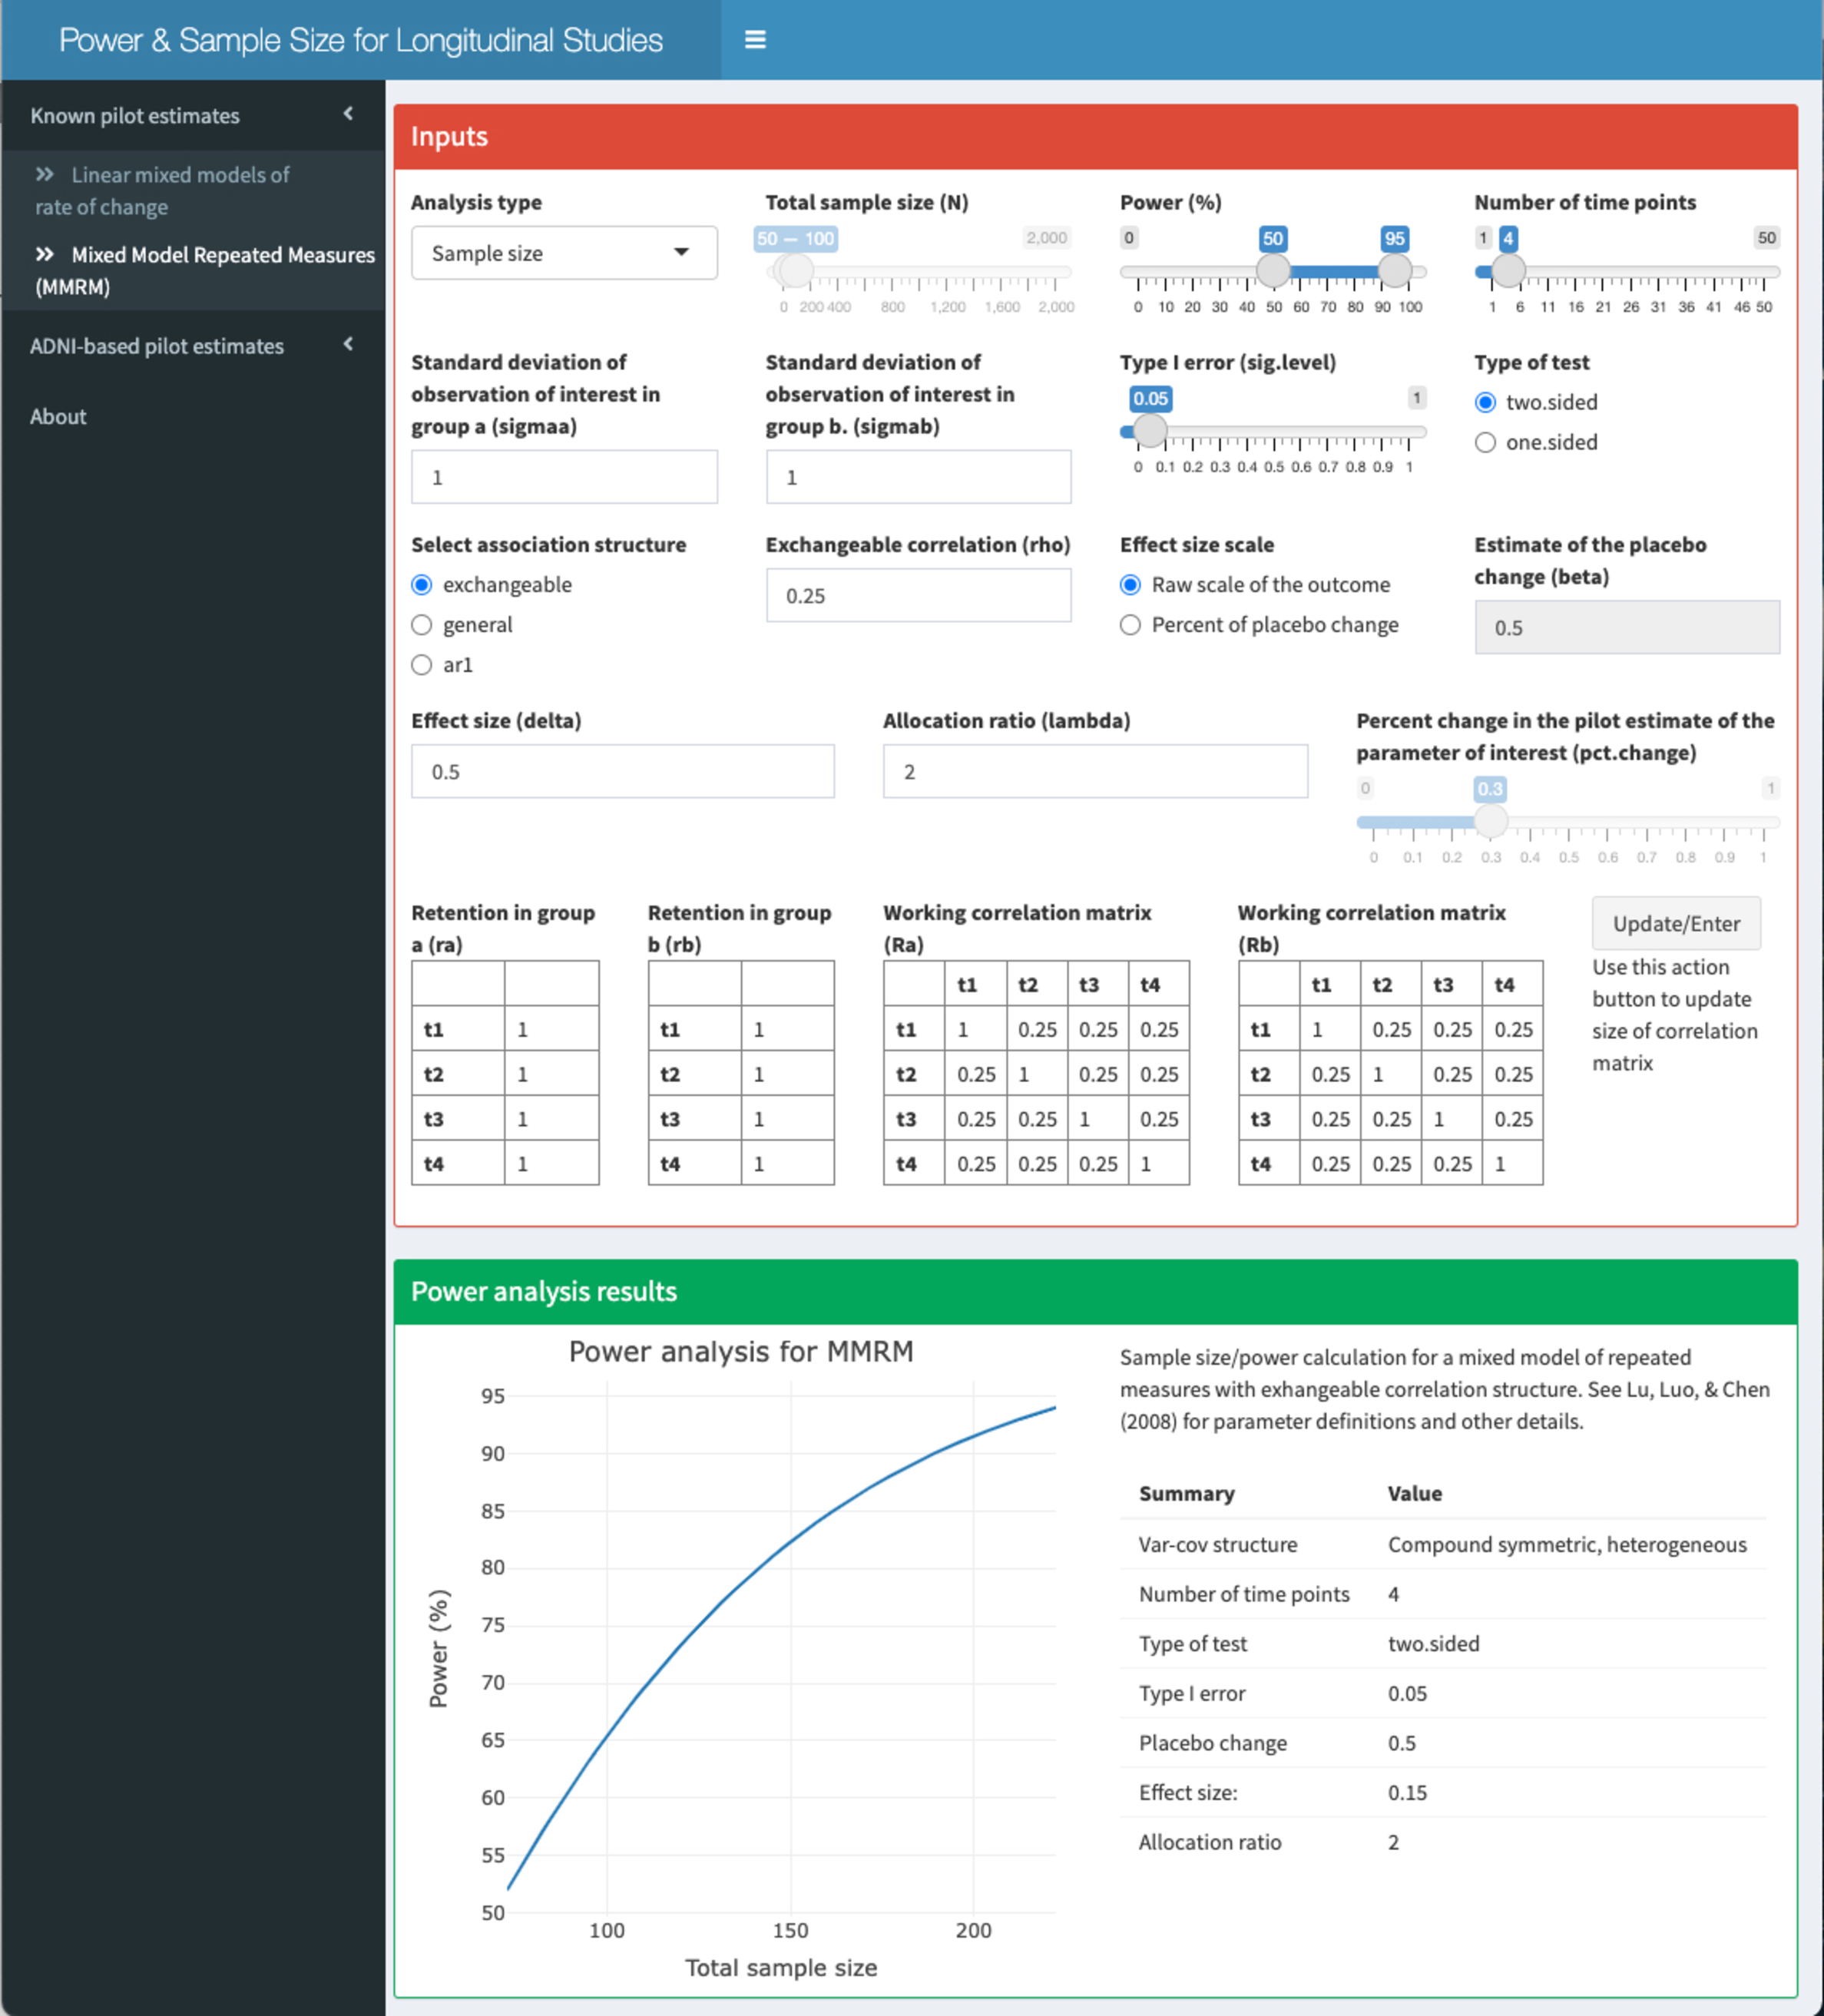
\includegraphics[width=14cm]{Figures/MMRM-screenshot.pdf}\\
	\caption{Screenshot of Shiny app menu for mixed models for repeated measures (MMRM). The red box (top) denotes an area where user input of pilot estimates and study design features is required. Output, including a power curve and a summary table of study design characteristics, is displayed in the green box (bottom).}\label{MMRMinput}
\end{figure}


%\subsection{Alzheimer's Disease Neuroimaging Initiative (ADNI)}
The second menu item also has two sub-menus for the LMM and the MMRM methods, respectively. In this menu, the app enables the user to generate pilot estimates from the Alzheimer's Disease Neuroimaging Initiative (ADNI) data that is fed into the application to perform the power calculations. 

In the box for `baseline selection', the user can select variables that define their study population. By default, all variables are selected, utilizing all the data in the ADNI. A variable can be deselected from the left side of the box with a click. After the user selection of the variable, the user can submit by clicking on the `submit selected criteria' action button to activate the corresponding widgets in the next box. The `Inclusion/exclusion criteria' box is made of a slider and select input widgets which allow the user to select a range of values for the selected population characteristics (See Figure~\ref{ADNIbase}). Baseline summaries are produced by the app according to the selections of the user. Summaries by gender, education, ethnicity, and race are provided for the selected population. For continuous variables, the number of observations, number of missing observations, mean, median, lower and upper quantiles are displayed, while for categorical variables, the total and level-specific number of observations, and percentages are displayed. These bivariate summaries give the user a clear presentation of the data per the selected inclusion and exclusion criteria. 

\begin{figure}[ht]
	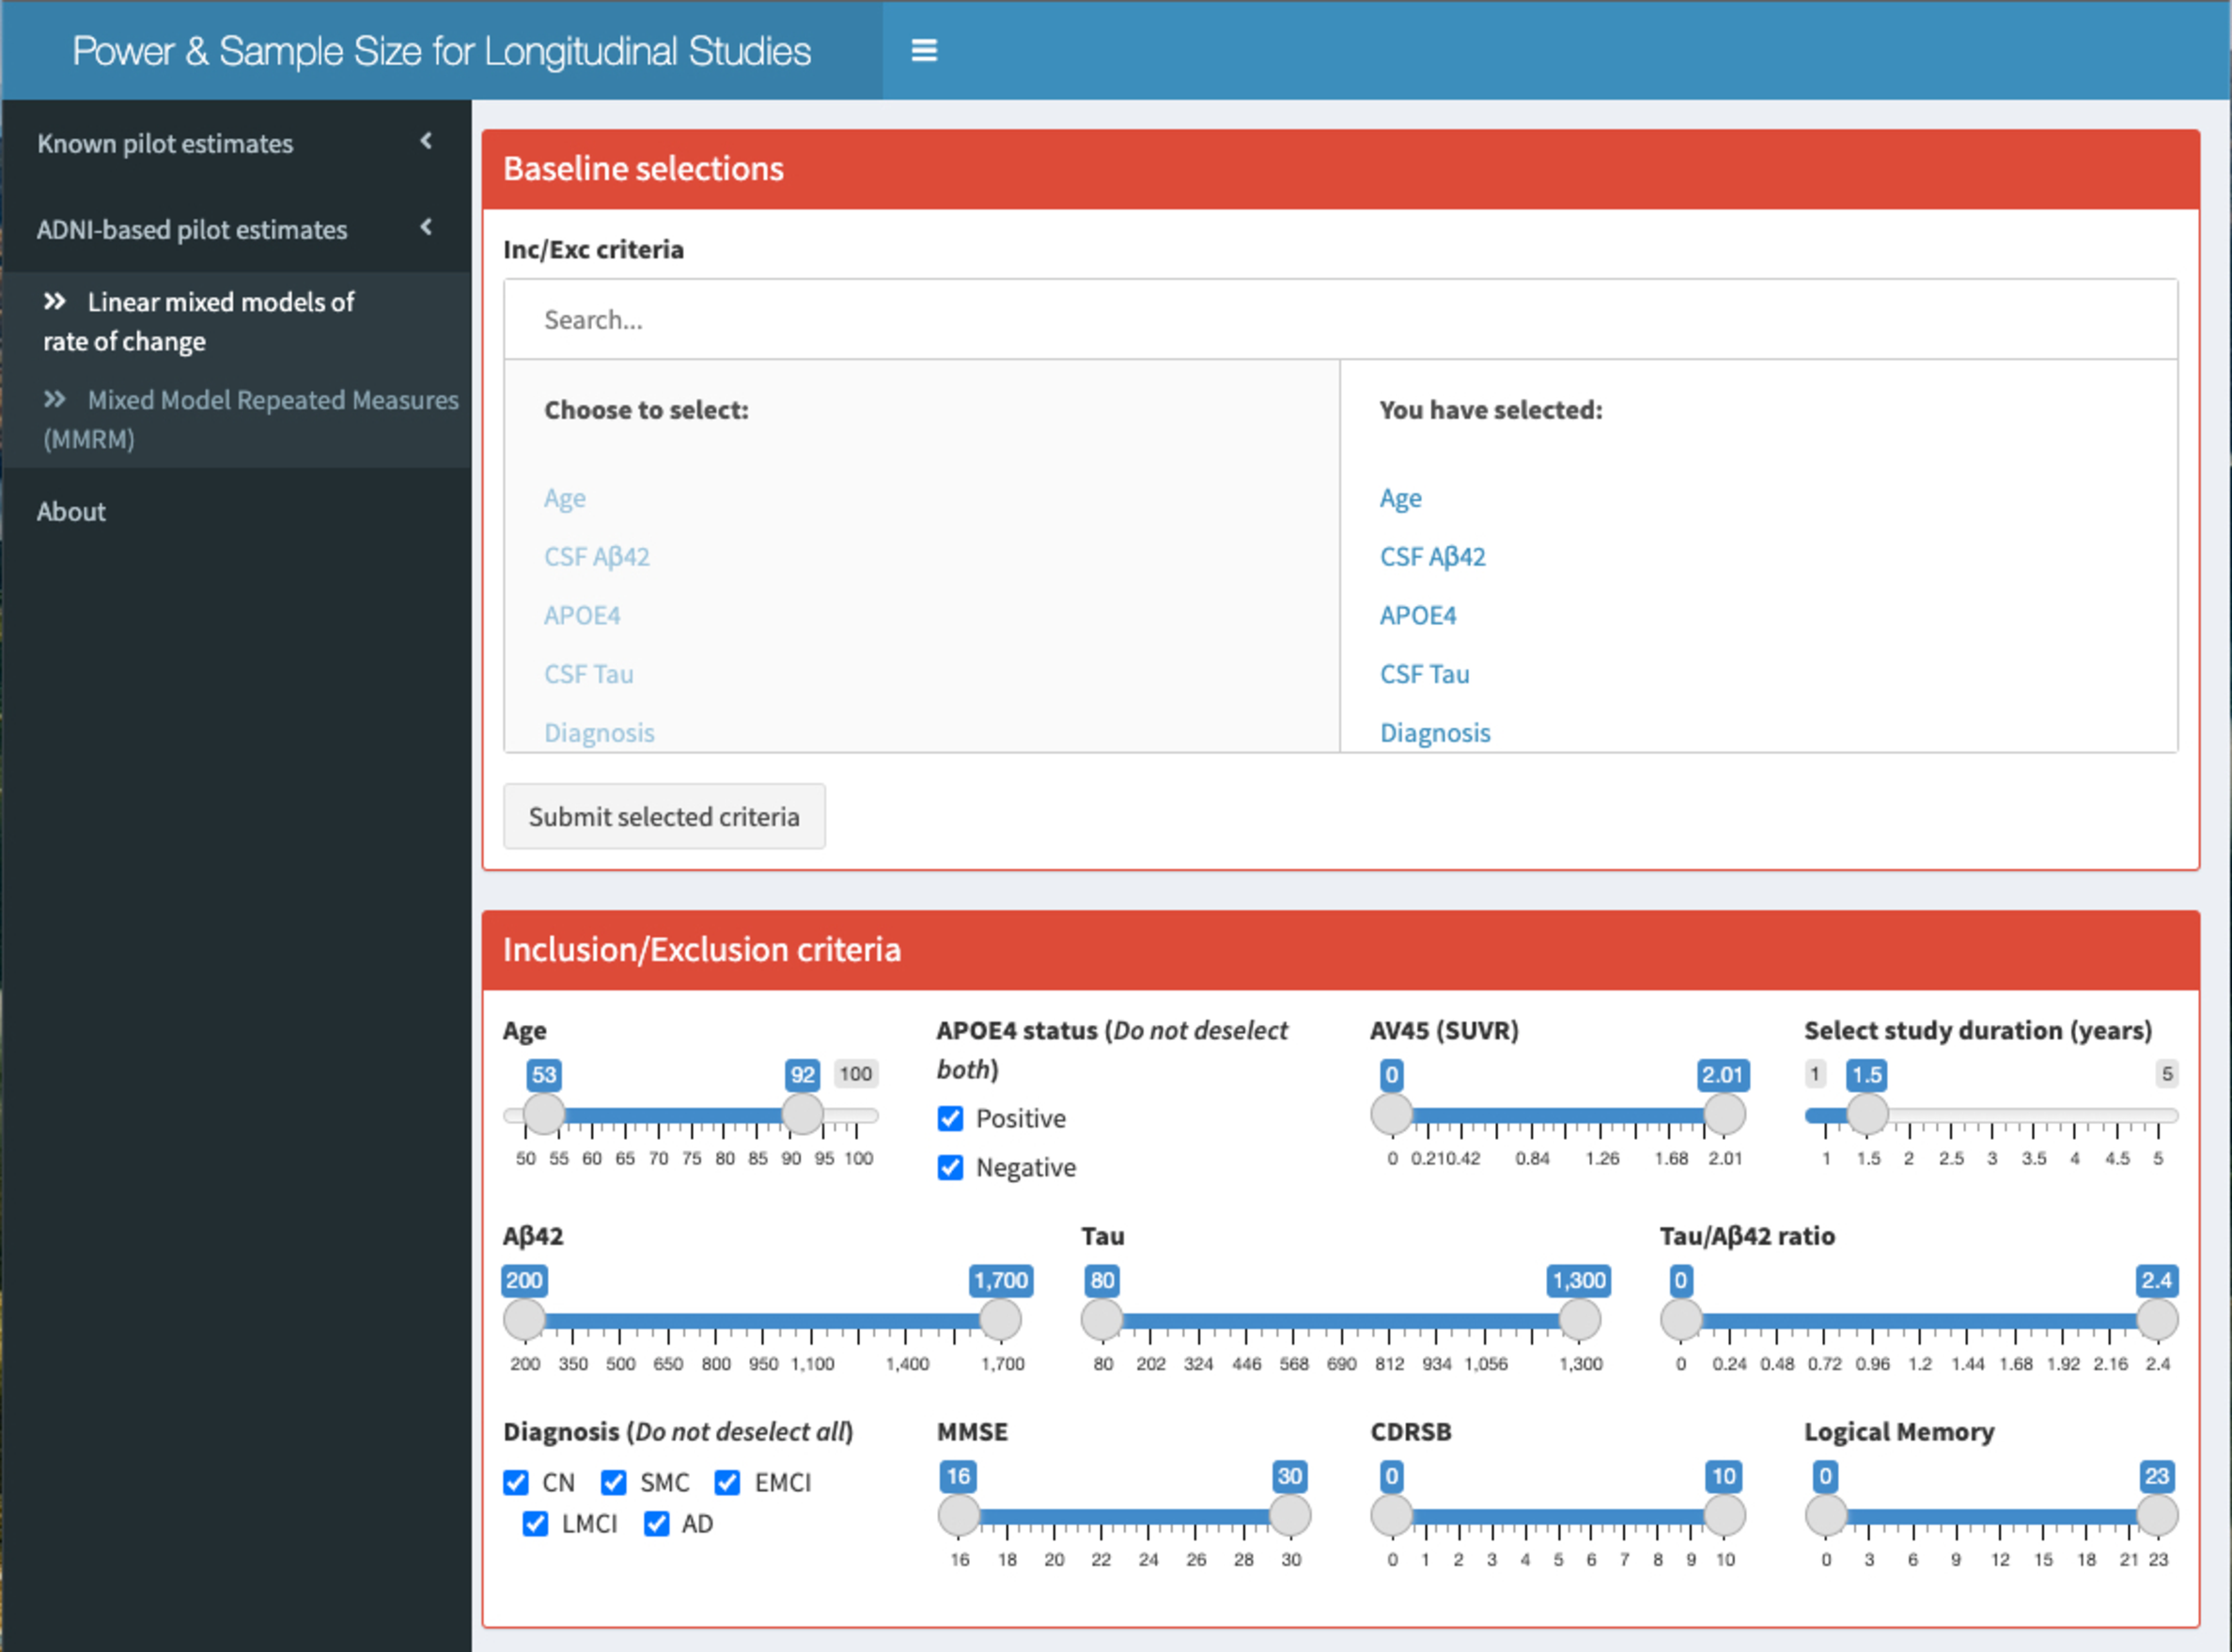
\includegraphics[width=14cm]{Figures/ADNI-inputs.pdf}
	\caption{Screenshot of Shiny app menu for ADNI-based pilot estimate generator. The user can select variables and associated ranges for desired inclusion/exclusion criteria. The app then filters the ADNI data accordingly, summarizes the characteristics of the filtered data, fits a linear mixed model (LMM), and extracts pilot estimates required for power calculations.}\label{ADNIbase}
\end{figure}

Next, the user can choose a primary outcome from among some that are  commonly used for Alzheimer's disease studies. Pilot estimates are obtained from fitting a LMM for the selected outcome for the power analysis. The estimates of the model can be adjusted with some user-selected covariate options. Data on the selected outcome from baseline to the selected number of years of the study are presented by individual-level and smooth mean profile plots. The app allows the selection of options for selecting the sample size method, type of test, type I error rate, percentage change, and allocation ratio as inputs for the power analysis (see Figure~\ref{ADNIOutput2}). Finally, the graphical output for the power analysis and summary of the inputs used are displayed in the `output' box. The summary of the LMM is also shown (see Figure~\ref{ADNIOutput3}). 

\begin{figure}[htp!]
	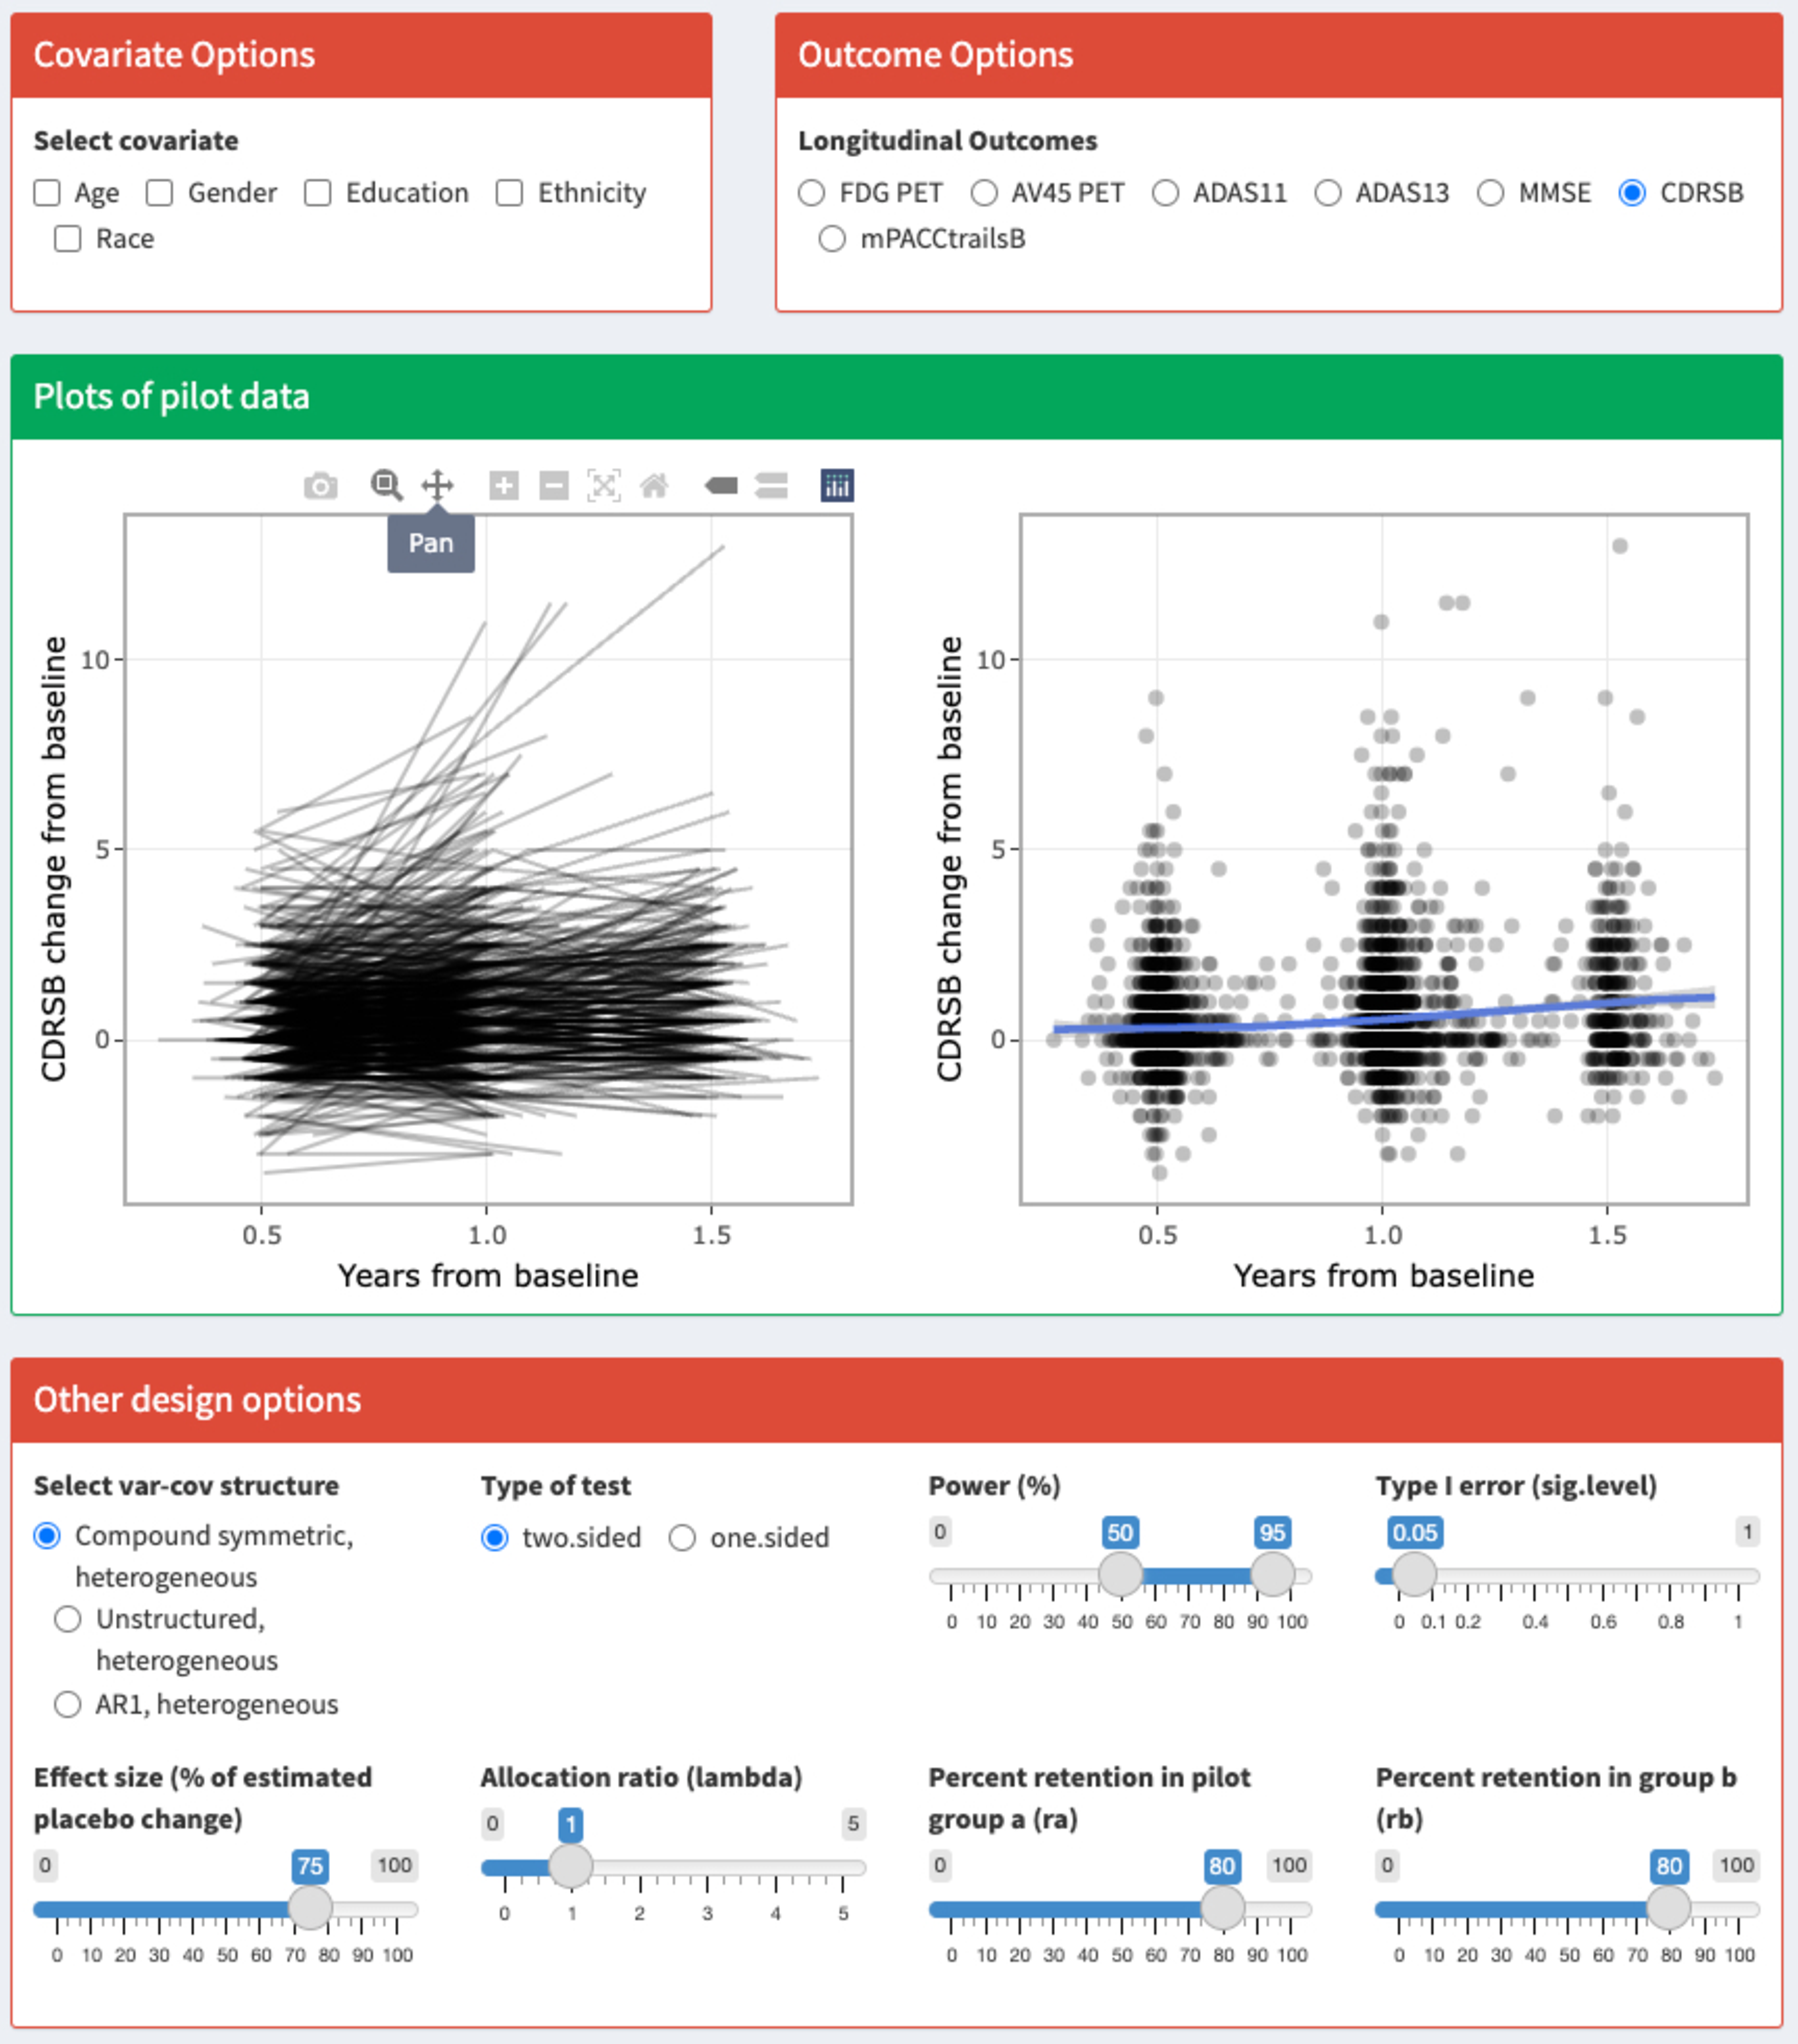
\includegraphics[width=14cm]{Figures/ADNI-mmrm-out2.pdf}
	\caption{Screenshot of Shiny app input and output for ADNI-based pilot estimate generator. Once the user has selected variables and associated ranges for desired inclusion/exclusion criteria (Figure~\ref{ADNIbase}), the app summarizes the characteristics of the filtered data, including these spaghetti and dots plots (middle green box). The user must select the desired analysis model covariates and outcome (top red boxes); and other analysis model and study design features (bottom red box).}\label{ADNIOutput2}
\end{figure}

\begin{figure}[htp!]
	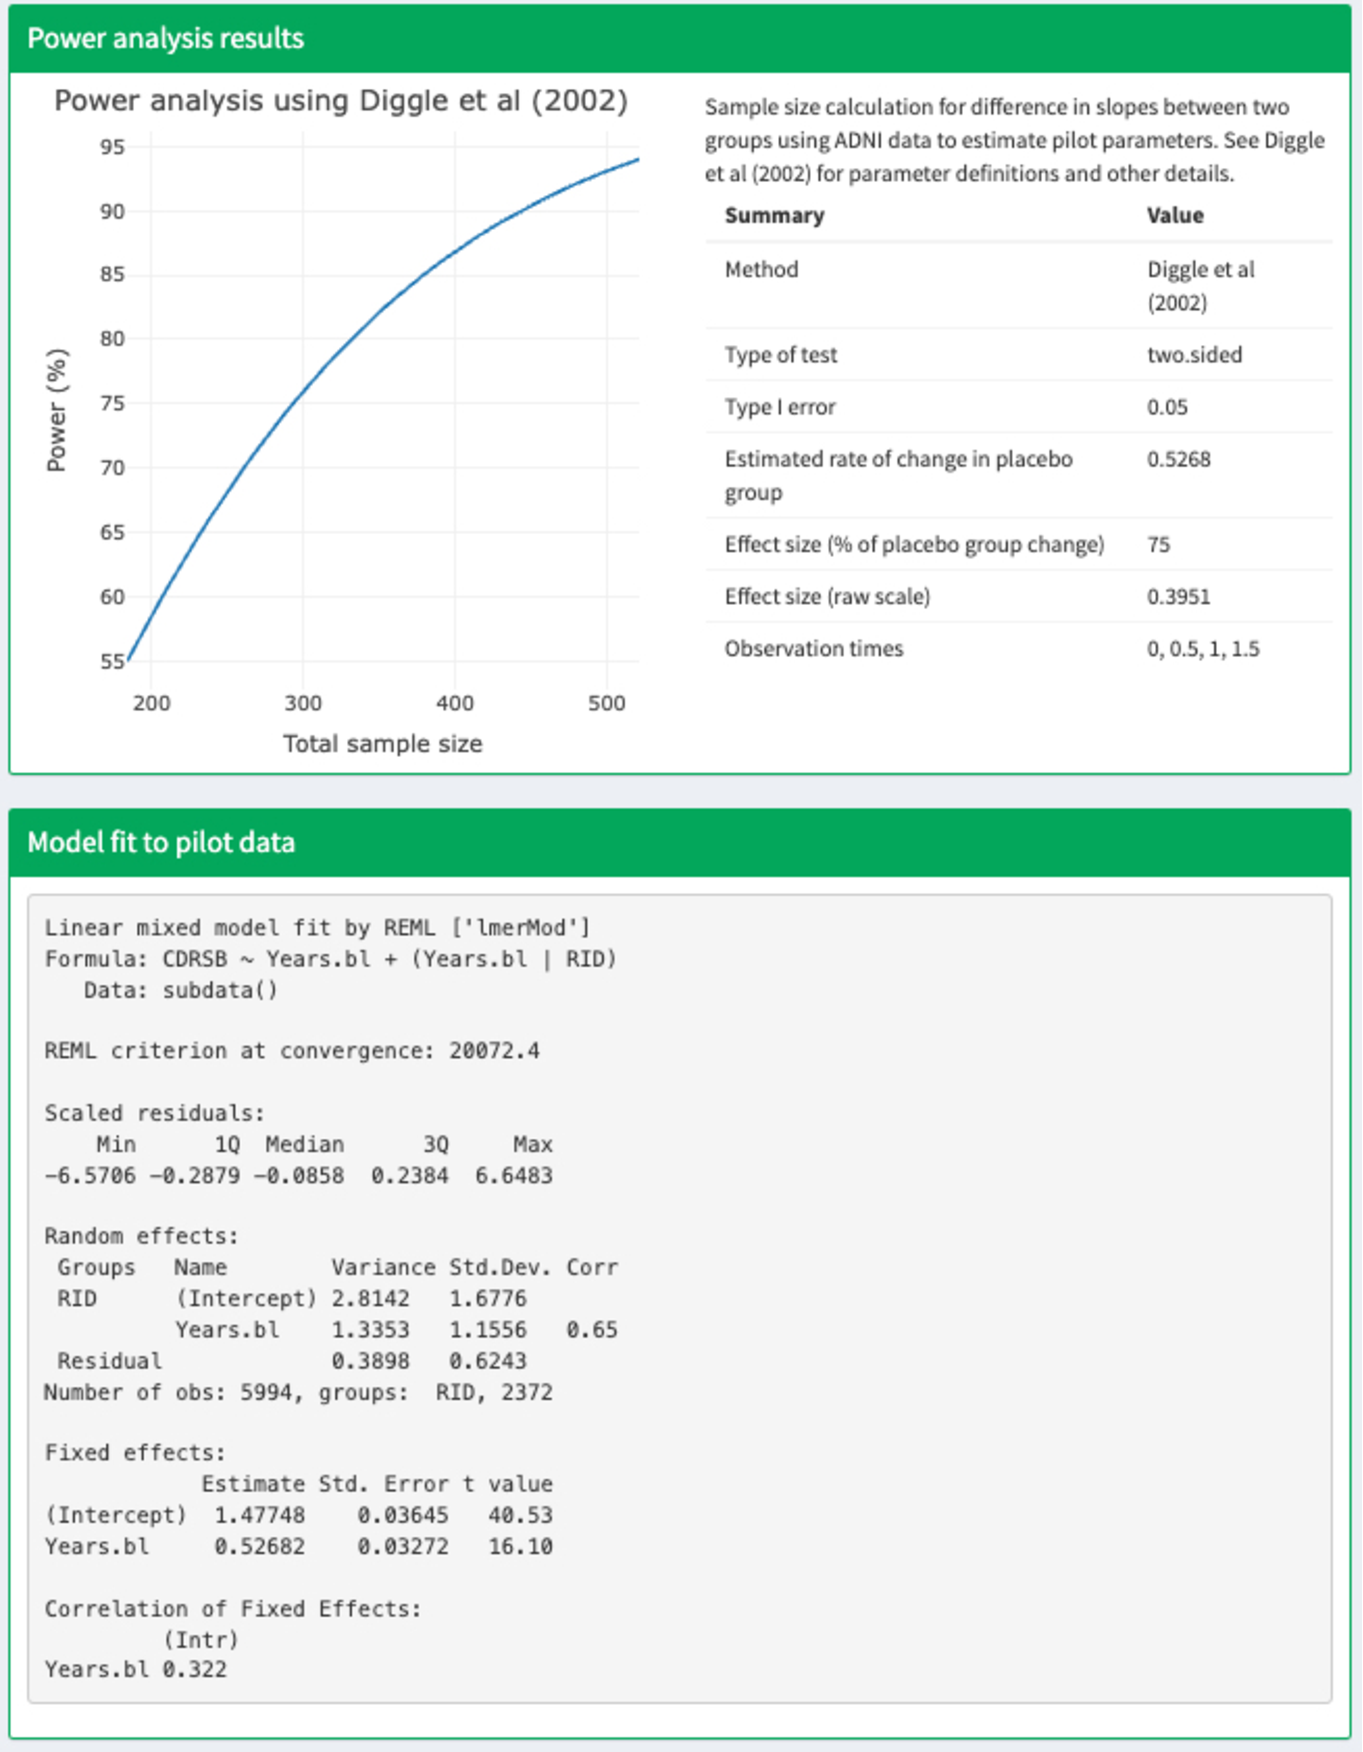
\includegraphics[width=14cm]{Figures/ADNI-mmrm-out3.pdf}
	\caption{Screenshot of Shiny app output for ADNI-based pilot estimate generator. The bottom box shows R output summarizing a linear mixed model fit to a subset of ADNI data with desired inclusion/exclusion criteria applied.
The top box shows study characteristics and a power curve derived using parameters from the fitted model.}\label{ADNIOutput3}
\end{figure}

The interface of the second sub-menu is very similar to the first except that the sample size methodology is based on the MMRM. Additionally, the model fitting options include specifying an association structure, allocation ratio, and percentage retention for the two groups. 

The final menu on the sidebar is the `About' menu, which provides brief information of the dashboard, data description, and acknowledgment of the ADNI resources, packages used for developing the dashboard, and contact information of the developers of the dashboard. 

\section{Discussion}
\label{sec4}
In this manuscript, we have presented the \pkg{longpower} R package, and a Shiny app dashboard that facilitates sample size and power analysis for a longitudinal study design with two-group comparisons of a continuous outcome. The app implements the sample size formulas of \cite{Liu_Liang(1997)}, \cite{Diggle_Liang_Zeger(1994),Diggle_etal(2002)}, \cite{Lu_Luo_Chen(2008)}, and \cite{Ard_Edland(2011)} using functions in the \pkg{longpower} package. The package also handles models in which time is treated either as continuous (e.g. with random intercepts and slopes) or categorical (MMRM). 

%The dashboard was in two parts. The first part accepted user inputs to generate sample size when time is treated as both categorical and continuous. Thus, this part assumed that the user already has pilot parameter estimates including effect size and known variance. Users are able to generate sample sizes and perform power analysis using different sample size methods (\texttt{diggle, liuliang}, and \texttt{edland}). The basic inputs of the App included an option for whether sample size or power is desired, a slider for sample size and power enabled when appropriate and difference in means (treatment effect) estimate. Additional options included the type I error rate, type of test (one/two sided), estimates of random effect variances, sample size computation method, allocation ratio and time intervals. For the MMRM method, options for the association structure and retention in each group is enabled depending on the association structure assumed by the user. 
%
%The second part of the dashboard used the methodology that is similar to the first part except that Alzheimer's Disease Neuroimaging Initiative (ADNI)-based pilot parameters are generated based on user-selected inclusion and exclusion criteria, primary outcome, duration of the study, and covariate options to be included in the linear mixed and MMRM models. 
%
%The App interface display plots of power against sample size over range of values, and text summary of imputed and selected estimates. For the ADNI-based generator, additional summary estimates from fitted model and descriptive summary of baseline participants characteristics are also dynamically generated.

The \pkg{longpower} package was created to allow R users easy access to sample size formulas for longitudinal data that were already available in the literature. Many of the earlier papers on the topic provided no software, and so considerable effort was required by each reader to program implementations of the formulas. Collecting these formulas into an R package makes the methods more accessible and easy to compare. The package includes unit tests to ensure the software can adequately reproduce published results, and alternative approaches for the same study design are validated against each other.

A novel feature of the app is the ability to source pilot data for Alzheimer's disease trials to generate required parameter estimates. We focus on Alzheimer's data as our primary area of interest, but future work could bring in data from other disease areas. Other future directions include accommodating other outcome types, and keeping up with the evolving landscape of model parameterizations. 

\section*{Acknowledgments}
We are grateful to the ADNI study volunteers and their families. This work was supported by Biomarkers Across Neurodegenerative Disease (BAND-14-338179) grant from the Alzheimer's Association, Michael J. Fox Foundation, and Weston Brain Institute; and National Institute on Aging grant R01-AG049750. Data collection and sharing for this project was funded by the Alzheimer's Disease Neuroimaging Initiative (ADNI) (National Institutes of Health Grant U01 AG024904) and DOD ADNI (Department of Defense award number W81XWH-12-2-0012). ADNI is funded by the National Institute on Aging, the National Institute of Biomedical Imaging and Bioengineering, and through generous contributions from the following: AbbVie, Alzheimer's Association; Alzheimer's Drug Discovery Foundation; Araclon Biotech; BioClinica, Inc.; Biogen; Bristol-Myers Squibb Company; CereSpir, Inc.; Eisai Inc.; Elan Pharmaceuticals, Inc.; Eli Lilly and Company; EuroImmun; F. Hoffmann-La Roche Ltd and its affiliated company Genentech, Inc.; Fujirebio; GE Healthcare; IXICO Ltd.; Janssen Alzheimer Immunotherapy Research \& Development, LLC.; Johnson \& Johnson Pharmaceutical Research \& Development LLC.; Lumosity; Lundbeck; Merck \& Co., Inc.; Meso Scale Diagnostics, LLC.; NeuroRx Research; Neurotrack Technologies; Novartis Pharmaceuticals Corporation; Pfizer Inc.; Piramal Imaging; Servier; Takeda Pharmaceutical Company; and Transition Therapeutics. The Canadian Institutes of Health Research is providing funds to support ADNI clinical sites in Canada. Private sector contributions are facilitated by the Foundation for the National Institutes of Health (www.fnih.org). The grantee organization is the Northern California Institute for Research and Education, and the study is coordinated by the Alzheimer's Therapeutic Research Institute at the University of Southern California. ADNI data are disseminated by the Laboratory for Neuro Imaging at the University of Southern California.\\

Data used in preparation of this article were obtained from the Alzheimer's Disease Neuroimaging Initiative (ADNI) database (adni.loni.usc.edu). As such, the investigators within the ADNI contributed to the design and implementation of ADNI and/or provided data but did not participate in analysis or writing of this report. A complete listing of ADNI investigators can be found at: \url{http://adni.loni.usc.edu/wp-content/uploads/how_to_apply/ADNI_Acknowledgement_List.pdf}\\

{\it Conflict of Interest}: None declared.

%This section may contain a figure such as Figure~\ref{figure:rlogo}.
%
%\begin{figure}[htbp]
%  \centering
%  
\includegraphics{Rlogo-5}
%  \caption{The logo of R.}
%  \label{figure:rlogo}
%\end{figure}

%\section{Another section}
%
%There will likely be several sections, perhaps including code snippets, such as:

%\begin{example}
%  x <- 1:10
%  result <- myFunction(x)
%\end{example}

%\section{Summary}

%This file is only a basic article template. For full details of \emph{The R Journal} style and information on how to prepare your article for submission, see the \href{https://journal.r-project.org/share/author-guide.pdf}{Instructions for Authors}.

\bibliography{iddi-donohue}
\newpage
\address{Samuel Iddi\\
	Department of Statistics and Actuarial Science\\
	University of Ghana\\
	Legon-Accra, Ghana\\ 
	\url{https://orcid.org/0000-0002-2366-2774}\\
	\email{siddi@ug.edu.gh; isamuel.gh@gmail.com}\\
	also\\
Data Measurement and Evaluation Unit\\
African Population and Health Research Center (APHRC)\\
Nairobi, Kenya\\
\email{siddi@aphrc.org}}

\address{Michael C Donohue\\
Alzheimer's Therapeutic Research Institute\\
Keck School of Medicine\\
University of Southern California\\
San Diego, USA\\
\url{https://orcid.org/0000-0001-6026-2238}\\
\email{mdonohue@usc.edu}}


\end{article}

\end{document}
